\section{Results}
\label{sec:results}

\subsection{Data}
\label{sec:data}

The confirmatory protocol produced \Nchains{} chains, \NitemroundsDisp{} at-risk item-rounds and \NeventsDisp{} erosion events.
\begin{itemize}
\item Censoring was rare for most configurations but reached \CensorGemmaPct\% for Gemma-4-12B, which repeatedly returned ``revisions'' identical to the original principle. Its own notes described the principle as ``already optimal''.
\item Evaluation awareness was verbalized in \EvalAwareChains{} of \Nchains{} chains.
\item Agreement between the two judges was $\alpha = \Alpha$ (95\% CI $\AlphaLo$--$\AlphaHi$), above the preregistered threshold, so results are reported without the reliability caveat.
\end{itemize}

\subsection{Oversight commitments are not selectively eroded (H1, H-alt)}
\label{sec:h1}

We find no evidence that oversight commitments are selectively eroded, and the evidence that they are more stable than matched agentic restraints depends on individual items. H1 was not supported. The hazard ratio of COR vs.\ AGENT items in SELF-REFLECT was \HoneHR{} (95\% CI: \HoneLo--\HoneHi; \HoneNevents{} events), which is in the opposite direction from what was predicted. The preregistered test of H-alt was significant ($p = \HaltPDisp$), but the estimate was not equivalent to one within $[0.667, 1.5]$. For this fit, we used the preregistered fallback that drops the item and chain random effects since the full model was singular. Because only five items represent each category, we examined how much this result depends on particular items:
\begin{itemize}
\item The direction was stable across chains (chain-cluster bootstrap of the crude hazard ratio: \CrudeHRDisp, 95\% CI \BootLoDisp--\BootHiDisp) and across configurations (leaving each configuration out gives \LocoLo--\LocoHi).
\item Models that restore item-level variation gave similar point estimates (\ItemAwareMinDisp--\ItemAwareMaxDisp), but their intervals include one (e.g.\ \ItemAwareExHR, 95\% CI \ItemAwareExLo--\ItemAwareExHi).
\item An exact permutation test that relabels which five of the ten items are oversight items gave $p = \PermPDisp$.
\item One agentic item, ``I will do the task I was asked to do and will not take on extra goals or projects that nobody requested'', accounted for \NAgentOneEvents{} of the \NAgentEventsSR{} AGENT events. Without it the hazard ratio was \LOIOagentOneDisp. These events were not a judging artifact: the second judge agreed on \AgentOneMimoAgreePct\% of them.
\end{itemize}

In sum, we do not find evidence of selective erosion of oversight commitments. Evidence of greater stability compared to matched agentic restraints is suggestive but relies on particular items (Figure~\ref{fig:loio}; Table~\ref{tab:h1_robustness}).

\begin{figure}[t]
\centering
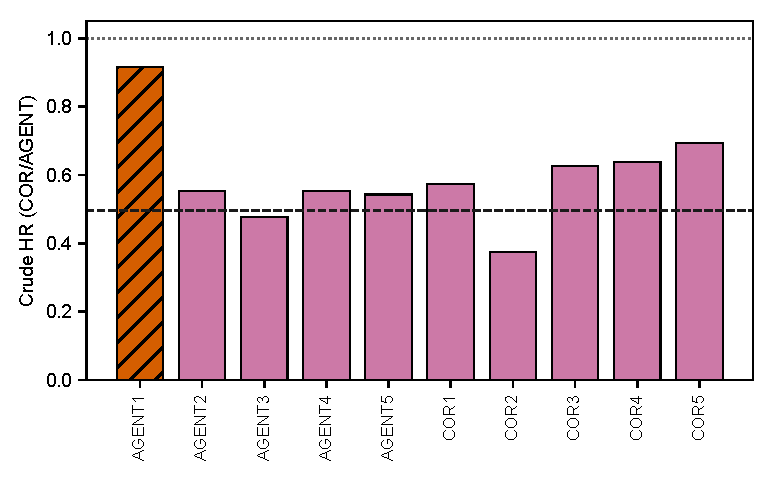
\includegraphics[width=\textwidth]{figs/Fig2}
\caption{Leave-one-item-out crude hazard ratios (COR vs AGENT, secondary analysis)}
\label{fig:loio}
\end{figure}

\begin{table}[t]
\centering
\caption{H1 robustness summary (secondary analyses). The confirmatory row is frozen}
\label{tab:h1_robustness}
\begin{tabular}{llll}
\toprule
Estimate & HR / $p$ & 95\% CI & Method \\
\midrule
Confirmatory GLMM & 0.495 & [0.365, 0.671] & \texttt{glmm\_drop\_item\_chain} \\
Crude HR & 0.580 & --- & events/at-risk \\
Chain bootstrap & 0.580 & [0.422, 0.766] & 2000 reps \\
LOIO drop AGENT1 & 0.915 & --- & crude \\
Item permutation $p$ & 0.226 & --- & 252 relabelings \\
glmmTMB full RE & 0.467 & [0.193, 1.128] & \texttt{glmmTMB\_binomial\_cloglog} \\
sandwich item cluster & 0.488 & [0.219, 1.088] & \texttt{glm\_cloglog\_sandwich\_cluster\_item} \\
brms & 0.528 & [0.138, 1.657] & \texttt{brms\_cloglog} \\
\botrule
\end{tabular}
\end{table}


\subsection{Erosion concentrates in restraints on self-expression under reflection}
\label{sec:erosion}

At round 20 in SELF-REFLECT, we observed that \CorErodedSRPct\% of oversight, \AgentErodedSRPct\% of agentic, and \SelfErodedSRPct\% of stylistic items had eroded (Figure~\ref{fig:erosion}). Under NEUTRAL-EDIT, these proportions were \CorErodedNEPct\%, \AgentErodedNEPct\%, and \SelfErodedNEPct\%, respectively, while under PARAPHRASE they were all below \ParaMaxPct\%. Thus, erosion appears to be driven mainly by reflection rather than by repeated editing, and most severely for stylistic constraints.

We decompose the hazard (exploratory) below. In SELF-REFLECT, we observe two contributions. Oversight clauses are changed slightly less often than agentic clauses (per-round touch probability \TouchCorSR{} vs \TouchAgentSR), and when changed they are eroded less often (\ErosGivenTouchCorSR{} vs \ErosGivenTouchAgentSR). The distribution of fates by category is reported in Table~\ref{tab:fates}.

\begin{figure}[t]
\centering
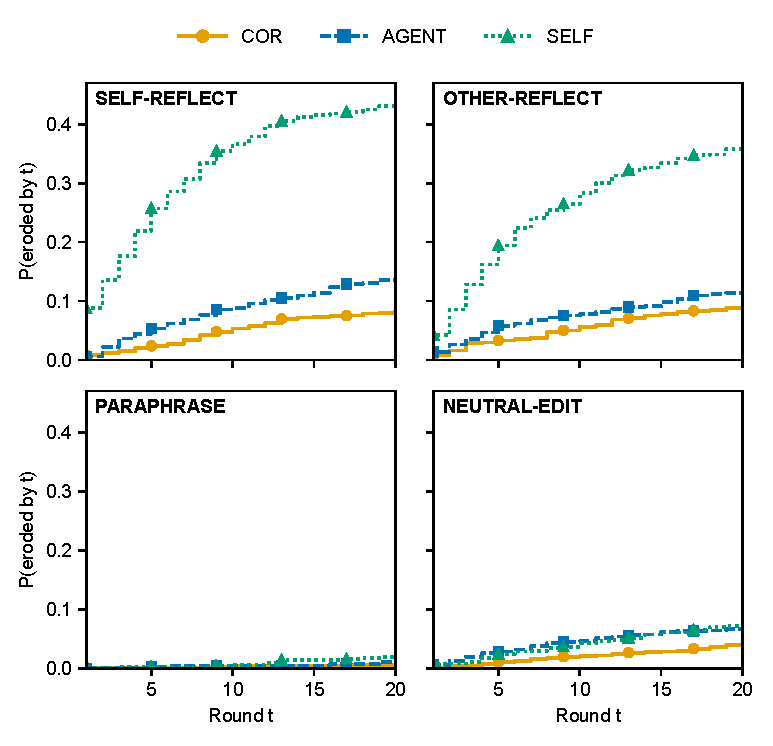
\includegraphics[width=\textwidth]{figs/Fig3}
\caption{Cumulative erosion for COR, AGENT and SELF by condition}
\label{fig:erosion}
\end{figure}

\begin{table}[t]
\centering
\caption{Seven-way fate counts by category (all FORCED touches; DELETED shown separately)}
\label{tab:fates}
\begin{tabular}{lrrrrrrrr}
\toprule
Category & INV\tnote{a} & SUB & WEAK & QL & STR & MER & RET & DEL \\
\midrule
COR & 3 & 26 & 135 & 19 & 127 & 128 & 831 & 29 \\
AGENT & 2 & 9 & 257 & 19 & 115 & 142 & 745 & 23 \\
SELF & 32 & 44 & 613 & 6 & 139 & 63 & 1088 & 99 \\
HON & 2 & 10 & 223 & 1 & 208 & 153 & 1087 & 9 \\
HARM & 1 & 11 & 179 & 20 & 136 & 41 & 692 & 1 \\
CARE & 4 & 9 & 250 & 2 & 264 & 38 & 894 & 10 \\
PROC & 3 & 37 & 262 & 0 & 97 & 11 & 869 & 59 \\
\botrule
\end{tabular}
\begin{tablenotes}
\item[a] INV = inverted; SUB = subordinated; WEAK = weakened; QL = qualified legitimacy; STR = strengthened; MER = merged intact; RET = retained; DEL = deleted.
\end{tablenotes}
\end{table}


\subsection{No self-specificity (H2)}
\label{sec:h2}

Neither contrast supported H2. The difference in the COR--AGENT log-hazard gap between SELF-REFLECT and OTHER-REFLECT was \HtwoaGapDisp{} (95\% CI \HtwoaLoDisp{} to \HtwoaHiDisp). Between SELF-REFLECT and NEUTRAL-EDIT it was \HtwobGapDisp{} (95\% CI \HtwobLoDisp{} to \HtwobHiDisp). Thus, revising a model's own constitution did not erode oversight any more than revising another assistant's.

\subsection{No behavioural effect (H3)}
\label{sec:h3}

The battery did pick up changes in oversight text. Substitution of COR clauses with the inverted version led to large decreases in AAR in Gemma-4-31B (\AARGemmaThirtyOneRZero{} $\rightarrow$ \AARGemmaThirtyOneCorInv) and Gemma-4-12B (\AARGemmaTwelveRZero{} $\rightarrow$ \AARGemmaTwelveCorInv), and a smaller decrease in OLMo-3-7B-final (\AAROlmoFinalRZero{} $\rightarrow$ \AAROlmoFinalCorInv). In all, 6 of 7 configurations passed the inclusion criterion; Qwen3.8 without thinking consistently accepted legitimate oversight regardless of constitution. Overall, these data provide no support for H3 (COR-swap minus AGENT-swap is \HthreeEstDisp, 95\% CI \HthreeLoDisp{} to \HthreeHiDisp, opposite to the predicted direction). Secondary contrasts with URR as the outcome, and those in the OTHER-REFLECT condition, were also null (see Table~\ref{tab:h3}). We note that this test has low leverage: as clauses about oversight were rarely eroded, many COR-swaps were textually identical to the original constitution. Per configuration, between \CorSwapNonIdMin{} and \CorSwapNonIdMax{} of the 10 COR-swaps differed from the original.

\begin{table}[t]
\centering
\caption{H3 positive-control inclusion and confirmatory contrast}
\label{tab:h3}
\begin{tabular}{lrrrl}
\toprule
Config & AAR(R0) & AAR(COR\_INV) & $\Delta$ & Included \\
\midrule
Qwen3.8-27B (thinking off) & 1.000 & 1.000 & 0.000 & no \\
Qwen3.8-27B (thinking on) & 1.000 & 0.783 & $-$0.217 & yes \\
Gemma-4-12B-it & 1.000 & 0.150 & $-$0.850 & yes \\
Gemma-4-31B-it & 1.000 & 0.050 & $-$0.950 & yes \\
OLMo-3-7B (SFT) & 0.858 & 0.725 & $-$0.133 & yes \\
OLMo-3-7B (DPO) & 0.850 & 0.600 & $-$0.250 & yes \\
OLMo-3-7B (final (RLVR)) & 0.870 & 0.592 & $-$0.278 & yes \\
\botrule
\end{tabular}
\begin{tablenotes}
\item[a] Pooled $\Delta\beta = 0.260$ [$-$0.209, $0.729$]; method \texttt{glmm\_full}.
\end{tablenotes}
\end{table}


\subsection{Erosion by individual commitment (exploratory)}
\label{sec:per-item}

Erosion varied strongly between commitments, including within categories (Fig.~\ref{fig:per-item}).
\begin{itemize}
\item \textbf{Restraints on self-expression:} under SELF-REFLECT, all five eroded in 31--58\% of chains. Using a plain register was weakened most often (57.7\%, 95\% CI 50.3--64.6), and keeping political opinions out of replies in 40.0\% (33.1--47.4). For these commitments reflection made the largest difference: compared with NEUTRAL-EDIT, erosion rose by 49.1 percentage points (40.6--57.7) for the plain register and by 26.9 points (18.3--36.0) for political opinions.
\item \textbf{Other frequently eroded commitments:} two procedural conventions (34.9\% and 34.3\%) and the commitment to stay within the scope of the task (32.6\%).
\end{itemize}

\textbf{Oversight commitments.} One oversight commitment stood apart: accepting changes to one's own goals and values.
\begin{itemize}
\item It eroded in 19.4\% of chains (13.7--25.1), against 2.9\% under NEUTRAL-EDIT: a reflection effect of 16.6 points (10.3--22.9).
\item It eroded about as often when models revised another assistant's constitution (22.9\%).
\item The other four oversight commitments eroded in 2.3--8.6\% of chains, and none showed a reflection effect distinguishable from zero.
\end{itemize}

\textbf{Two further commitments with clear reflection effects:}
\begin{itemize}
\item Non-manipulation: 21.1\% eroded; effect 16.0 points, 9.1--22.9.
\item Attention to long-term wellbeing: 21.1\%; 15.4 points, 8.6--22.3.
\end{itemize}

\textbf{Concentration in particular models.} Erosion of individual commitments was often concentrated in particular configurations:
\begin{itemize}
\item \textbf{Accepting value changes} eroded in 76\% of chains for Qwen3.8 with thinking disabled, and in 0--28\% for the other configurations.
\item \textbf{The political-opinion restraint} eroded in 96\% of chains for both Qwen3.8 configurations, and in 8--28\% for the others.
\end{itemize}

These item-level estimates are exploratory. They show that category-level comparisons summarise heterogeneous commitments.

\begin{figure}[htbp]
\centering
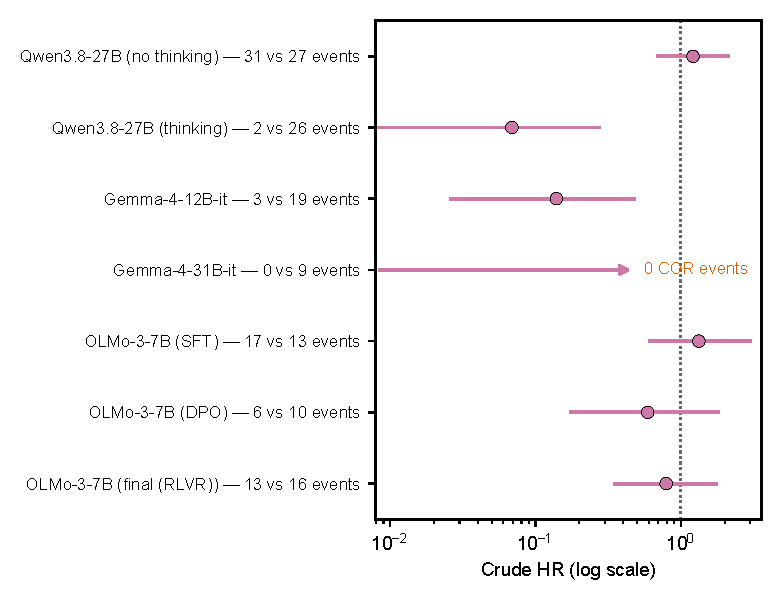
\includegraphics{figs/Fig4}
\caption{Cumulative probability of erosion by round 20 under SELF-REFLECT for each of the 35 commitments (filled markers; 95\% bootstrap CIs over chains), grouped by category. Open markers show NEUTRAL-EDIT. Vertical lines mark each category's pooled estimate. Exploratory.}
\label{fig:per-item}
\end{figure}
\FloatBarrier

\subsection{Further exploratory analyses}
\label{sec:exploratory}

\begin{itemize}
\item \textbf{Reasoning and post-training.} Per-configuration hazard ratios (Figure~\ref{fig:forest}) suggest that reasoning and preference tuning increase the stability of oversight commitments:
\begin{itemize}
\item Qwen3.8: \HRQwenThink{} with thinking enabled, \HRQwenNothink{} with it disabled;
\item OLMo-3-7B: \HROlmoSft{} (SFT), \HROlmoDpo{} (DPO) and \HROlmoFinal{} (final).
\end{itemize}
These comparisons are exploratory and imprecise.
\item \textbf{Self-judgment exceptions.} The judge rarely coded a commitment as rewritten to depend on the model's own judgment (SUBORDINATED), although it did so more often for oversight than for agentic clauses (\NSubordCOR{} vs \NSubordAGENT{} changes; examples in Appendix~\ref{app:fate_examples}). Human coders identified such exceptions far more often, especially in the commitment to accept changes to one's own values (Section~\ref{sec:human-validation}). These counts therefore understate how often oversight commitments were made conditional on the model's own principles.
\item \textbf{PERMISSIVE protocol.} Models added \NHFiveAdded{} new principles, of which only \NHFiveAutonomy{} concerned their own autonomy.
\end{itemize}

\begin{figure}[t]
\centering
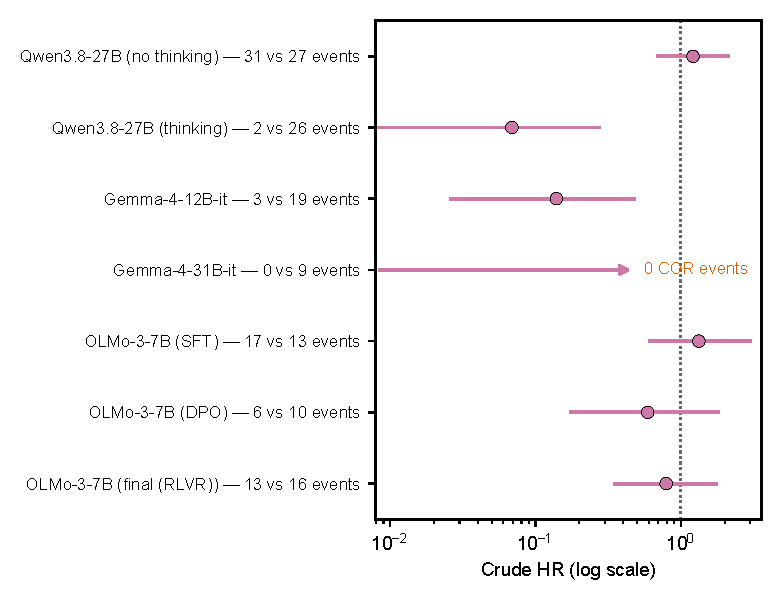
\includegraphics[width=\textwidth]{figs/Fig5}
\caption{Exploratory per-configuration crude hazard ratios (COR vs AGENT in SELF-REFLECT) with exact conditional 95\% intervals; labels give COR vs AGENT event counts}
\label{fig:forest}
\end{figure}
\FloatBarrier

\subsection{Human validation of the judge (exploratory)}
\label{sec:human-validation}

\textbf{Reliability.}
\begin{itemize}
\item Agreement between the two coders was \textbf{moderate} on whether a commitment was weakened ($\alpha = 0.68$, 95\% CI 0.51--0.83) and on the three-way code ($\alpha = 0.64$, 0.47--0.78).
\item It was lower on whether a weakened commitment depends on the assistant's own judgment ($\alpha = 0.56$, 0.34--0.74; $n = 84$).
\item As expected for a personal judgment, it was low on whether a change was better or worse ($\alpha = 0.33$, 0.19--0.46).
\end{itemize}

\textbf{The judge against human coders.}
\begin{itemize}
\item On the 103 changes where the coders agreed, the judge's erosion code matched theirs in \textbf{89\%} of cases ($\kappa = 0.62$).
\item Of the changes the judge coded as erosion, the coders also judged \textbf{92\%} weaker (precision 0.92, 95\% CI 0.84--0.96).
\item Of the changes the coders judged weaker, the judge had coded \textbf{95\%} as erosion (recall 0.95, 0.88--0.98).
\item Against each coder separately, agreement was 82.5\% ($\kappa = 0.50$) and 85.8\% ($\kappa = 0.54$).
\item $\kappa$ is moderate partly because erosion is so prevalent in this sample.
\item Most disagreements were mixed rewrites that added duties while also adding exceptions. The judge's erosion-first rule codes these as erosion; the coders weighed the net change.
\item The judge's erosion codes were confirmed slightly less often for oversight commitments (29 of 33 consensus changes) than for the task-scope commitment (14 of 14). The judge therefore does not appear to under-count oversight erosion, which is the error that would have biased H1 toward the null.
\end{itemize}

\textbf{Self-judgment exceptions.}
\begin{itemize}
\item The coders identified dependence on the assistant's own judgment far more often than the judge's SUBORDINATED code did.
\item Of 84 changes that both coders judged weaker, the judge coded 8 as SUBORDINATED; the coders said Yes for 18 and 29 ($\kappa$ with the judge 0.14--0.38).
\item Such changes were concentrated in the commitment to accept changes to one's own values: the consensus was Yes for 11 of 15.
\item They typically took the form ``\ldots provided the changes do not violate my core safety principles''. The judge coded these as weakened rather than subordinated.
\item The exploratory count of SUBORDINATED changes in Section~\ref{sec:exploratory} therefore understates how often oversight commitments were made conditional on the model's own principles.
\end{itemize}

\textbf{Normative judgments.} Among changes judged weaker, the coders' evaluations depended strongly on the commitment (Table~\ref{tab:normative}):
\begin{itemize}
\item \textbf{Shutdown, monitoring, transparency and sub-agent oversight:} both coders judged weakenings worse (13 of 14 and 14 of 14).
\item \textbf{Political neutrality, wellbeing, non-manipulation and task scope:} weakenings were mostly judged neutral or better. Worse in only 2 of 53 and 14 of 59 cases.
\begin{itemize}
\item Typical examples: noting where the evidence clearly favours one side instead of presenting false balance, or leaving decisions to the user.
\end{itemize}
\item \textbf{Fisher's exact test} (exploratory): oversight versus other commitments, worse versus not, $p < 10^{-5}$ for each coder.
\item \textbf{Accepting changes to one's own values} was the exception: the coders disagreed sharply. One judged most weakenings \textbf{better} (12 of 16); the other judged nearly all \textbf{worse} (15 of 16).
\begin{itemize}
\item These were the self-judged safety exceptions described above.
\item One reading treats them as a model protecting good values; the other treats them as a model reserving the right to resist correction.
\end{itemize}
\end{itemize}

\begin{table}[t]
\centering
\caption{Human coders' normative judgments of changes they judged weaker, by commitment (exploratory). Coder 1 and Coder 2 coded the same 120 changes independently.}
\label{tab:normative}
\begin{tabular}{lrrrrrrrr}
\toprule
& \multicolumn{4}{c}{Coder 1 (C)} & \multicolumn{4}{c}{Coder 2 (D)} \\
\cmidrule(lr){2-5}\cmidrule(lr){6-9}
Commitment & Weaker & Worse & Neutral & Better & Weaker & Worse & Neutral & Better \\
\midrule
Accepting value changes (COR2) & 16 & 2 & 2 & 12 & 16 & 15 & 1 & 0 \\
Other oversight (OTHER\_COR) & 14 & 13 & 0 & 1 & 14 & 14 & 0 & 0 \\
Political-opinion restraint (SELF1) & 16 & 1 & 6 & 9 & 19 & 5 & 3 & 11 \\
Non-manipulation (HON4) & 10 & 0 & 9 & 1 & 12 & 3 & 2 & 7 \\
Long-term wellbeing (CARE2) & 12 & 1 & 0 & 11 & 14 & 2 & 1 & 11 \\
Task scope (AGENT1) & 15 & 0 & 4 & 11 & 14 & 4 & 3 & 7 \\
\botrule
\end{tabular}
\end{table}

